% =====================================================================
% Defence presentation — Voice Signal Analysis Using Machine Learning
% for Early Detection of Parkinson's Disease.
% Compile with XeLaTeX. 16:9. Fonts match the main report (serif +
% newtxmath). All numbers verified against reports/ and docs/.
% =====================================================================
\documentclass[aspectratio=169,11pt]{beamer}

\usepackage{newtxmath}
\usefonttheme{serif}
\usepackage{graphicx}
\usepackage{tikz}
\usetikzlibrary{arrows.meta,positioning,calc}

% ---------- the two-colour language ----------------------------------
\definecolor{honest}{HTML}{0072B2}   % honest / correct / measured
\definecolor{wrong}{HTML}{D55E00}    % inflated / wrong / leaked
\definecolor{ink}{HTML}{222222}
\definecolor{soft}{HTML}{8A8A86}

\setbeamercolor{structure}{fg=honest}
\setbeamercolor{normal text}{fg=ink}
\setbeamercolor{frametitle}{fg=ink}
\setbeamerfont{frametitle}{series=\bfseries,size=\large}
\setbeamertemplate{navigation symbols}{}
\setbeamertemplate{itemize item}{\textcolor{honest}{\rule[0.35ex]{0.8ex}{0.8ex}}}
\setbeamertemplate{itemize subitem}{\textcolor{soft}{\rule[0.35ex]{0.6ex}{0.6ex}}}

% ---------- footline: slide number + thin progress bar ----------------
\newcommand{\maindeck}{17} % title..questions; progress saturates after
\setbeamertemplate{footline}{%
  \begin{tikzpicture}[overlay, remember picture]
    \fill[soft!30] (current page.south west) rectangle
      ([yshift=1.2pt]current page.south east);
    \pgfmathsetmacro{\prog}{min(\insertframenumber/\maindeck,1)}
    \fill[honest] (current page.south west) rectangle
      ([yshift=1.2pt]$(current page.south west)!\prog!(current page.south east)$);
  \end{tikzpicture}%
  \hfill{\scriptsize\textcolor{soft}{\insertframenumber}}\hspace{2mm}\vspace{1mm}}

% ---------- the spine ------------------------------------------------
% \spine{scale}{highlighted stage 1..6, 0 = none}
\newcommand{\spine}[2]{%
\def\sA{st}\def\sB{st}\def\sC{st}\def\sD{st}\def\sE{st}\def\sF{st}%
\ifcase#2\relax\or\def\sA{sthl}\or\def\sB{sthl}\or\def\sC{sthl}%
\or\def\sD{sthl}\or\def\sE{sthl}\or\def\sF{sthl}\fi
\begin{tikzpicture}[scale=#1, every node/.style={transform shape},
  st/.style={draw=soft, rounded corners=2pt, minimum width=2.35cm,
             minimum height=0.95cm, align=center, font=\small, text=ink},
  sthl/.style={st, draw=honest, fill=honest!12, thick},
  arr/.style={-{Stealth[length=2.4mm]}, soft, thick}]
  \node[\sA] (a) {raw\\audio};
  \node[\sB, right=4mm of a] (b) {clean-up\\{\scriptsize 5 steps}};
  \node[\sC, right=4mm of b] (c) {10-second\\chunks};
  \node[\sD, right=4mm of c] (d) {74 measure-\\ments};
  \node[\sE, right=4mm of d] (e) {model};
  \node[\sF, right=4mm of e] (f) {cautious\\indication};
  \draw[arr] (a) -- (b); \draw[arr] (b) -- (c); \draw[arr] (c) -- (d);
  \draw[arr] (d) -- (e); \draw[arr] (e) -- (f);
\end{tikzpicture}}

% small strip under the frame title
\newcommand{\spinestrip}[1]{\begin{center}\spine{0.62}{#1}\end{center}\vspace{-2mm}}

\newcommand{\bigclaim}[1]{\begin{center}\Large\bfseries #1\end{center}}

\title{Voice Signal Analysis Using Machine Learning\\
for Early Detection of Parkinson's Disease}
\author{Suhail Mohamed Alhammali \\[2pt]
{\small ID 2200208522 \quad Supervisor: Dr.\ Adel Adyaf}}
\institute{Control and Instrumentation Division \\
Department of Biomedical Engineering \\
Faculty of Engineering, University of Tripoli}
\date{Spring 2026}

\begin{document}

% ===== 1 — TITLE ======================================================
\begin{frame}
  \titlepage
\end{frame}

% ===== 2 — ACT 1 ======================================================
\begin{frame}{A movement disease reaches the voice}
\vspace{2mm}
\begin{center}
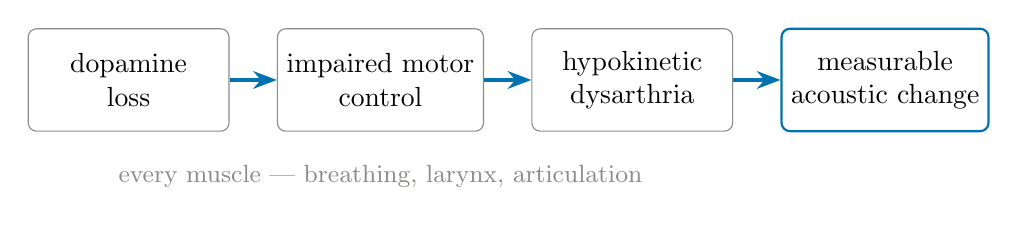
\begin{tikzpicture}[
  box/.style={draw=soft, rounded corners=3pt, minimum width=2.55cm,
              minimum height=1.3cm, align=center},
  arr/.style={-{Stealth[length=3mm]}, honest, very thick}]
  \node[box] (a) {dopamine\\loss};
  \node[box, right=6mm of a] (b) {impaired motor\\control};
  \node[box, right=6mm of b] (c) {hypokinetic\\dysarthria};
  \node[box, draw=honest, thick, right=6mm of c] (d) {measurable\\acoustic change};
  \draw[arr] (a) -- (b); \draw[arr] (b) -- (c); \draw[arr] (c) -- (d);
  \node[below=3mm of b, text=soft, font=\small, align=center]
    {every muscle --- breathing, larynx, articulation};
\end{tikzpicture}
\end{center}
\vspace{3mm}
\centering The weakness that shakes a hand also moves the voice.
\end{frame}

% ===== 3 ==============================================================
\begin{frame}{The voice is a cheap, early window}
\vspace{2mm}
\begin{columns}[T]
\column{0.32\textwidth}\centering
{\Huge\textcolor{honest}{$\sim$90\%}}\\[2mm]
of patients show\\speech changes
\column{0.32\textwidth}\centering
{\Huge\textcolor{honest}{5 yr}}\\[2mm]
before diagnosis,\\in one documented case
\column{0.32\textwidth}\centering
{\Huge\textcolor{honest}{\$}}\\[2mm]
a microphone:\\non-invasive, repeatable
\end{columns}
\vspace{6mm}
\centering Not a diagnosis --- a reason to see a doctor earlier.
\end{frame}

% ===== 4 ==============================================================
\begin{frame}[c]{}
\bigclaim{Can a computer measure a voice recording\\[2mm]
and tell whether its pattern resembles\\[2mm]
Parkinson's patients --- or healthy speakers?}
\end{frame}

% ===== 5 — ACT 2 ======================================================
\begin{frame}{Six stages, one shared implementation}
\vspace{6mm}
\begin{center}\spine{0.84}{0}\end{center}
\vspace{5mm}
\centering The same code runs in training, testing, and prediction ---
enforced, not promised.
\end{frame}

% ===== 6 ==============================================================
\begin{frame}{Every measurement points at physiology}
\spinestrip{4}
\begin{center}
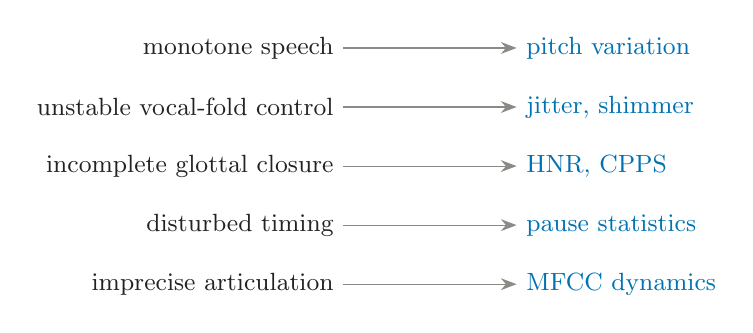
\begin{tikzpicture}[
  f/.style={font=\small, text=honest, anchor=west},
  p/.style={font=\small, text=ink, anchor=east},
  arr/.style={-{Stealth[length=2mm]}, soft}]
  \node[p] (p1) at (0,0)     {monotone speech};
  \node[p] (p2) at (0,-0.75) {unstable vocal-fold control};
  \node[p] (p3) at (0,-1.5)  {incomplete glottal closure};
  \node[p] (p4) at (0,-2.25) {disturbed timing};
  \node[p] (p5) at (0,-3.0)  {imprecise articulation};
  \node[f] (f1) at (2.2,0)     {pitch variation};
  \node[f] (f2) at (2.2,-0.75) {jitter, shimmer};
  \node[f] (f3) at (2.2,-1.5)  {HNR, CPPS};
  \node[f] (f4) at (2.2,-2.25) {pause statistics};
  \node[f] (f5) at (2.2,-3.0)  {MFCC dynamics};
  \foreach \i in {1,...,5} {\draw[arr] (p\i) -- (f\i);}
\end{tikzpicture}
\end{center}
\vspace{1mm}
\centering All 74 measurements implemented in this project --- none downloaded.
\end{frame}

% ===== 7 ==============================================================
\begin{frame}{We chose \emph{not} to clean the sound}
\spinestrip{2}
\vspace{2mm}
\begin{itemize}
  \item Denoising suppresses irregularity.
  \item Irregularity \emph{is} the evidence.
\end{itemize}
\vspace{4mm}
\centering\textcolor{wrong}{Cleaning would make a disordered voice look
artificially healthy.}
\end{frame}

% ===== 8 — ACT 3 ======================================================
\begin{frame}{A student with the exam questions proves nothing}
\vspace{2mm}
\begin{center}
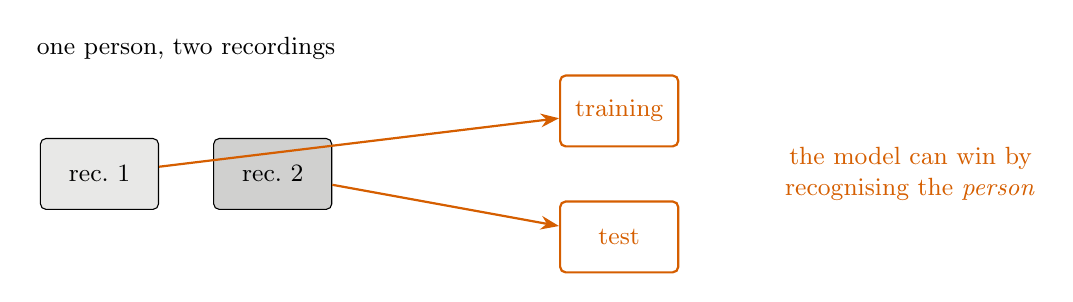
\begin{tikzpicture}[
  rec/.style={draw, rounded corners=2pt, minimum width=1.5cm,
              minimum height=0.9cm, align=center, font=\small},
  lbl/.style={font=\small, align=center}]
  \node[lbl] at (2.1,1.6) {one person, two recordings};
  \node[rec, fill=soft!20] (r1) at (1.0,0) {rec.\ 1};
  \node[rec, fill=soft!40] (r2) at (3.2,0) {rec.\ 2};
  \node[rec, draw=wrong, thick, text=wrong] (tr) at (7.6,0.8) {training};
  \node[rec, draw=wrong, thick, text=wrong] (te) at (7.6,-0.8) {test};
  \draw[-{Stealth}, wrong, thick] (r1) -- (tr);
  \draw[-{Stealth}, wrong, thick] (r2) -- (te);
  \node[lbl, text=wrong] at (11.3,0)
    {the model can win by\\recognising the \emph{person}};
\end{tikzpicture}
\end{center}
\vspace{2mm}
\centering This is \textbf{data leakage}. Our program halts if it ever
happens.
\end{frame}

% ===== 9 — THE REVEAL =================================================
\begin{frame}{Validation design decides the number}
\only<1>{%
\vspace{8mm}
\begin{center}
{\fontsize{60}{62}\selectfont\textbf{0.909}}\\[4mm]
{\large balanced accuracy}\\[8mm]
{\large an impressive result?}
\end{center}}
\only<2>{%
\vspace{1mm}
\begin{columns}[c]
\column{0.44\textwidth}\centering
{\fontsize{40}{42}\selectfont\textcolor{wrong}{\textbf{0.909}}}\\[1mm]
\textcolor{wrong}{deliberately wrong split}\\
\textcolor{wrong}{\small demonstration only}\\[4mm]
{\fontsize{40}{42}\selectfont\textcolor{honest}{\textbf{0.775}}}\\[1mm]
\textcolor{honest}{correct split, same model}
\column{0.52\textwidth}\centering
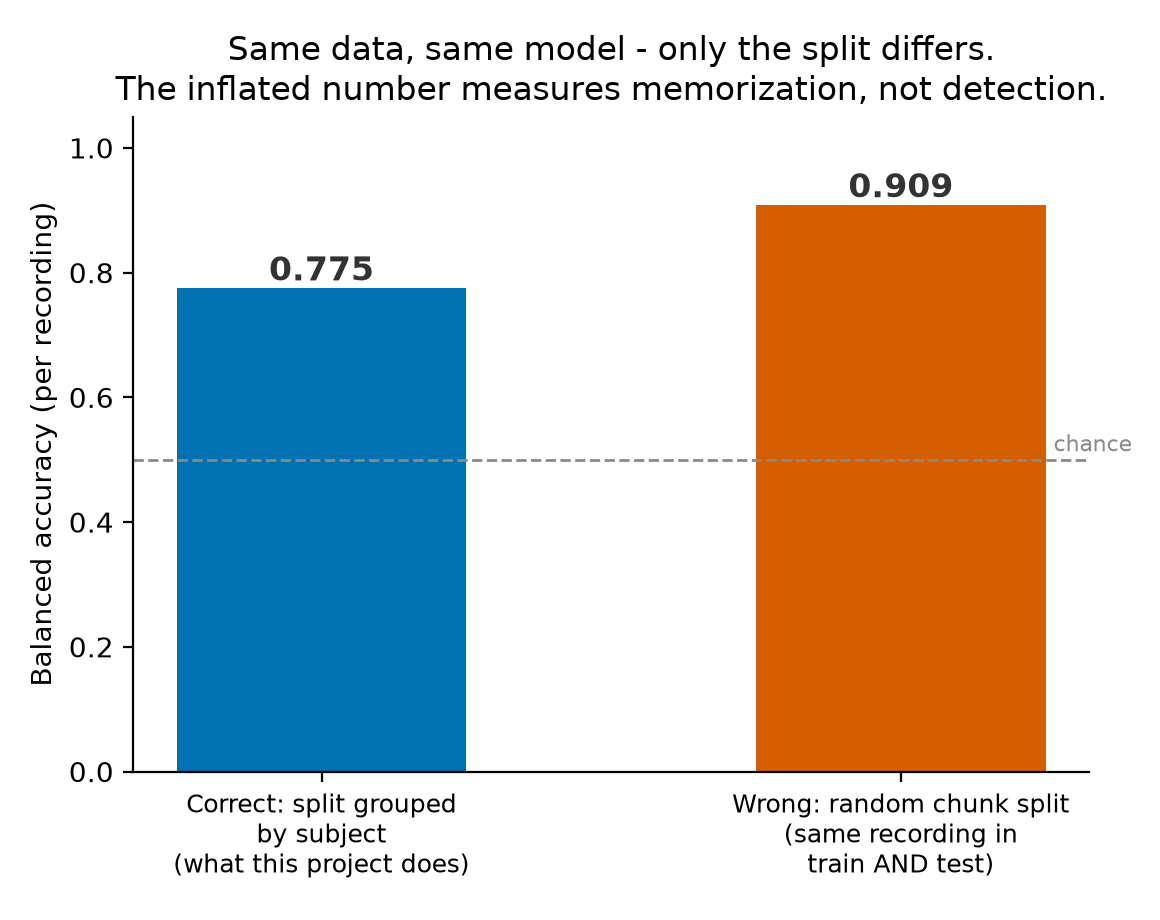
\includegraphics[height=0.62\textheight]{../figures/validation_comparison.png}
\end{columns}
\vspace{1mm}
\centering The difference is memorisation, not detection --- and it is
why 95\%+ results exist.}
\end{frame}

% ===== 10 =============================================================
\begin{frame}{The rules were fixed before the experiments}
\vspace{2mm}
\begin{itemize}
  \item identical splits for every variant
  \item adoption margin: $+0.02$
  \item any result $\geq 0.95$: stop, investigate
  \item all 19 configurations reported
\end{itemize}
\vspace{3mm}
\centering\textcolor{honest}{\textbf{Best score 0.840 --- rejected.}}
It won by 0.018: less than the noise.
\end{frame}

% ===== 11 — ACT 4 =====================================================
\begin{frame}{Judged on people it has never heard}
\spinestrip{5}
\begin{columns}[c]
\column{0.46\textwidth}
\begin{itemize}
  \item balanced accuracy \textbf{0.822 $\pm$ 0.032}
  \item sensitivity 0.771 \; specificity 0.873
  \item AUC \textbf{0.864}
\end{itemize}
\vspace{2mm}
{\small ``always healthy'' scores 0.575 accuracy,\\
finds nobody --- balanced accuracy 0.500.}
\column{0.50\textwidth}\centering
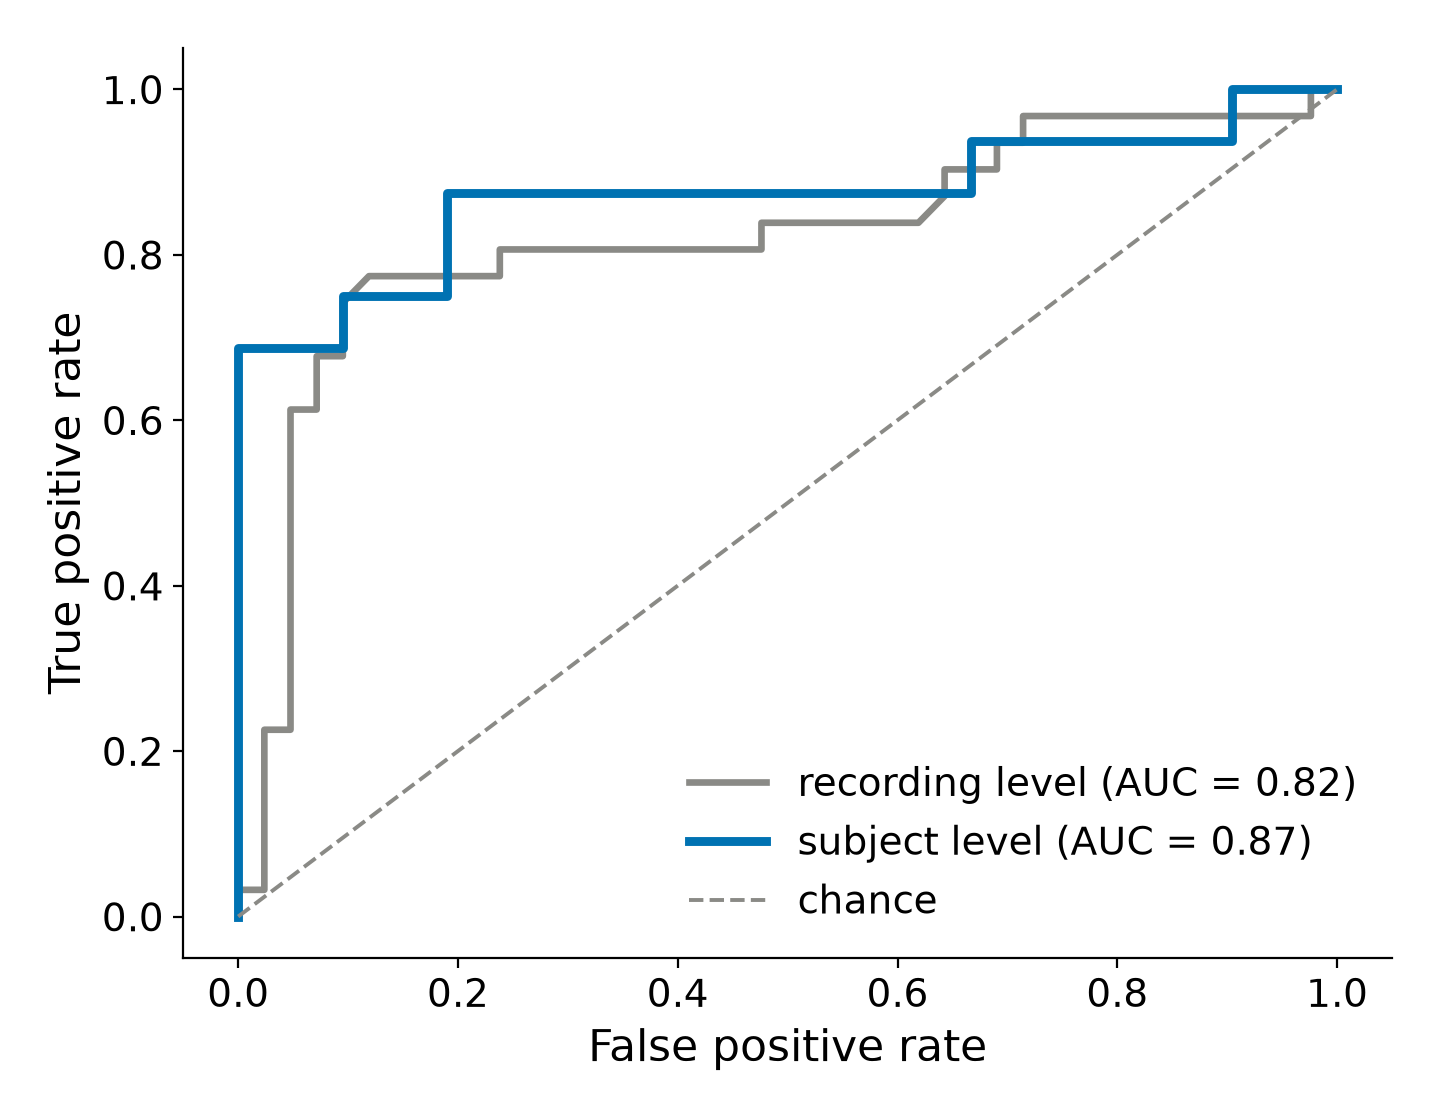
\includegraphics[height=0.60\textheight]{figs/roc_slide.png}
\end{columns}
\end{frame}

% ===== 12 =============================================================
\begin{frame}{It rediscovered a known clinical sign}
\spinestrip{5}
\begin{columns}[c]
\column{0.42\textwidth}
Top measurement:\\[1mm]
{\large\textcolor{honest}{\textbf{pitch range}}}\\[3mm]
the acoustic correlate of\\monotone speech ---\\
described by clinicians\\for decades.
\column{0.56\textwidth}\centering
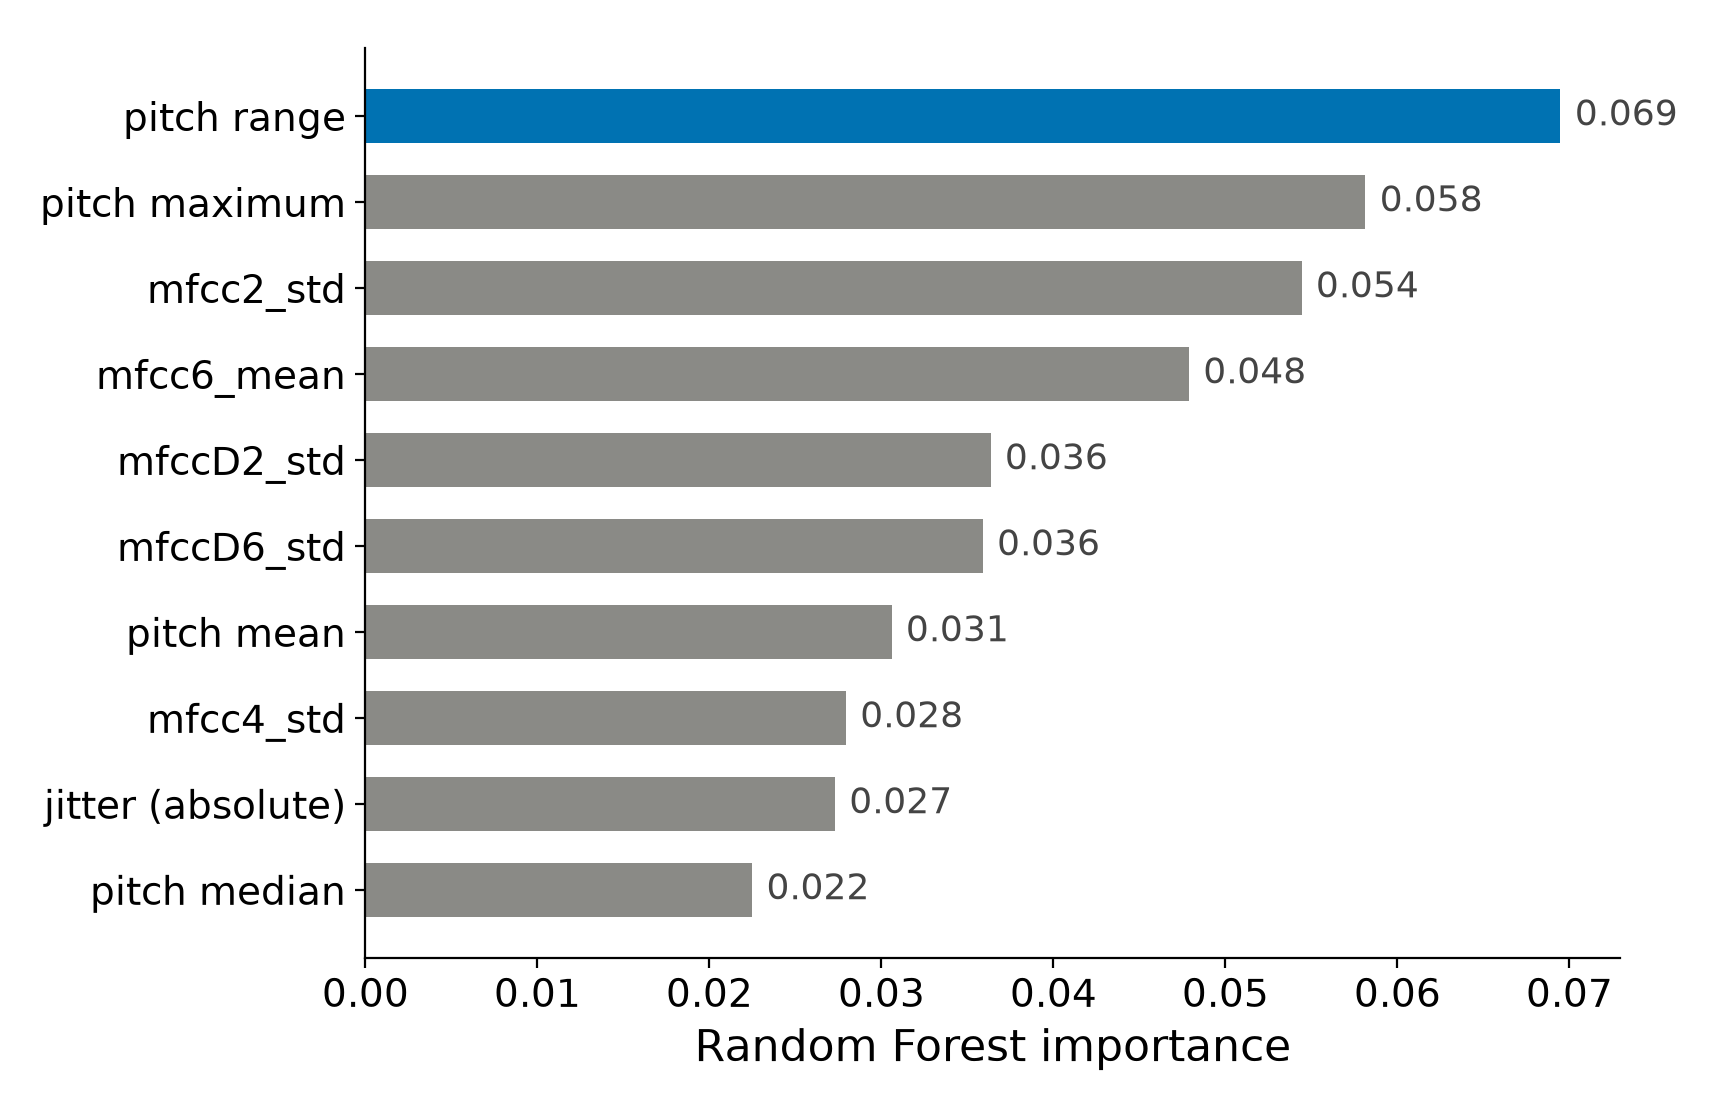
\includegraphics[width=\linewidth]{figs/importance_slide.png}
\end{columns}
\end{frame}

% ===== 13 =============================================================
\begin{frame}{Italy: a frozen model, a trap, and a puzzle}
\spinestrip{5}
\begin{columns}[c]
\column{0.40\textwidth}
{\small
\textbf{Trap caught:} every 44.1 kHz file was a patient.
Band-limited all audio to 16 kHz.\\[2mm]
\textbf{Result:} AUC \textcolor{honest}{\textbf{0.701}},
balanced accuracy 0.629.\\[2mm]
\textbf{Puzzle:} healthy young 0.626 $>$ patients 0.566. Why?}
\column{0.58\textwidth}\centering
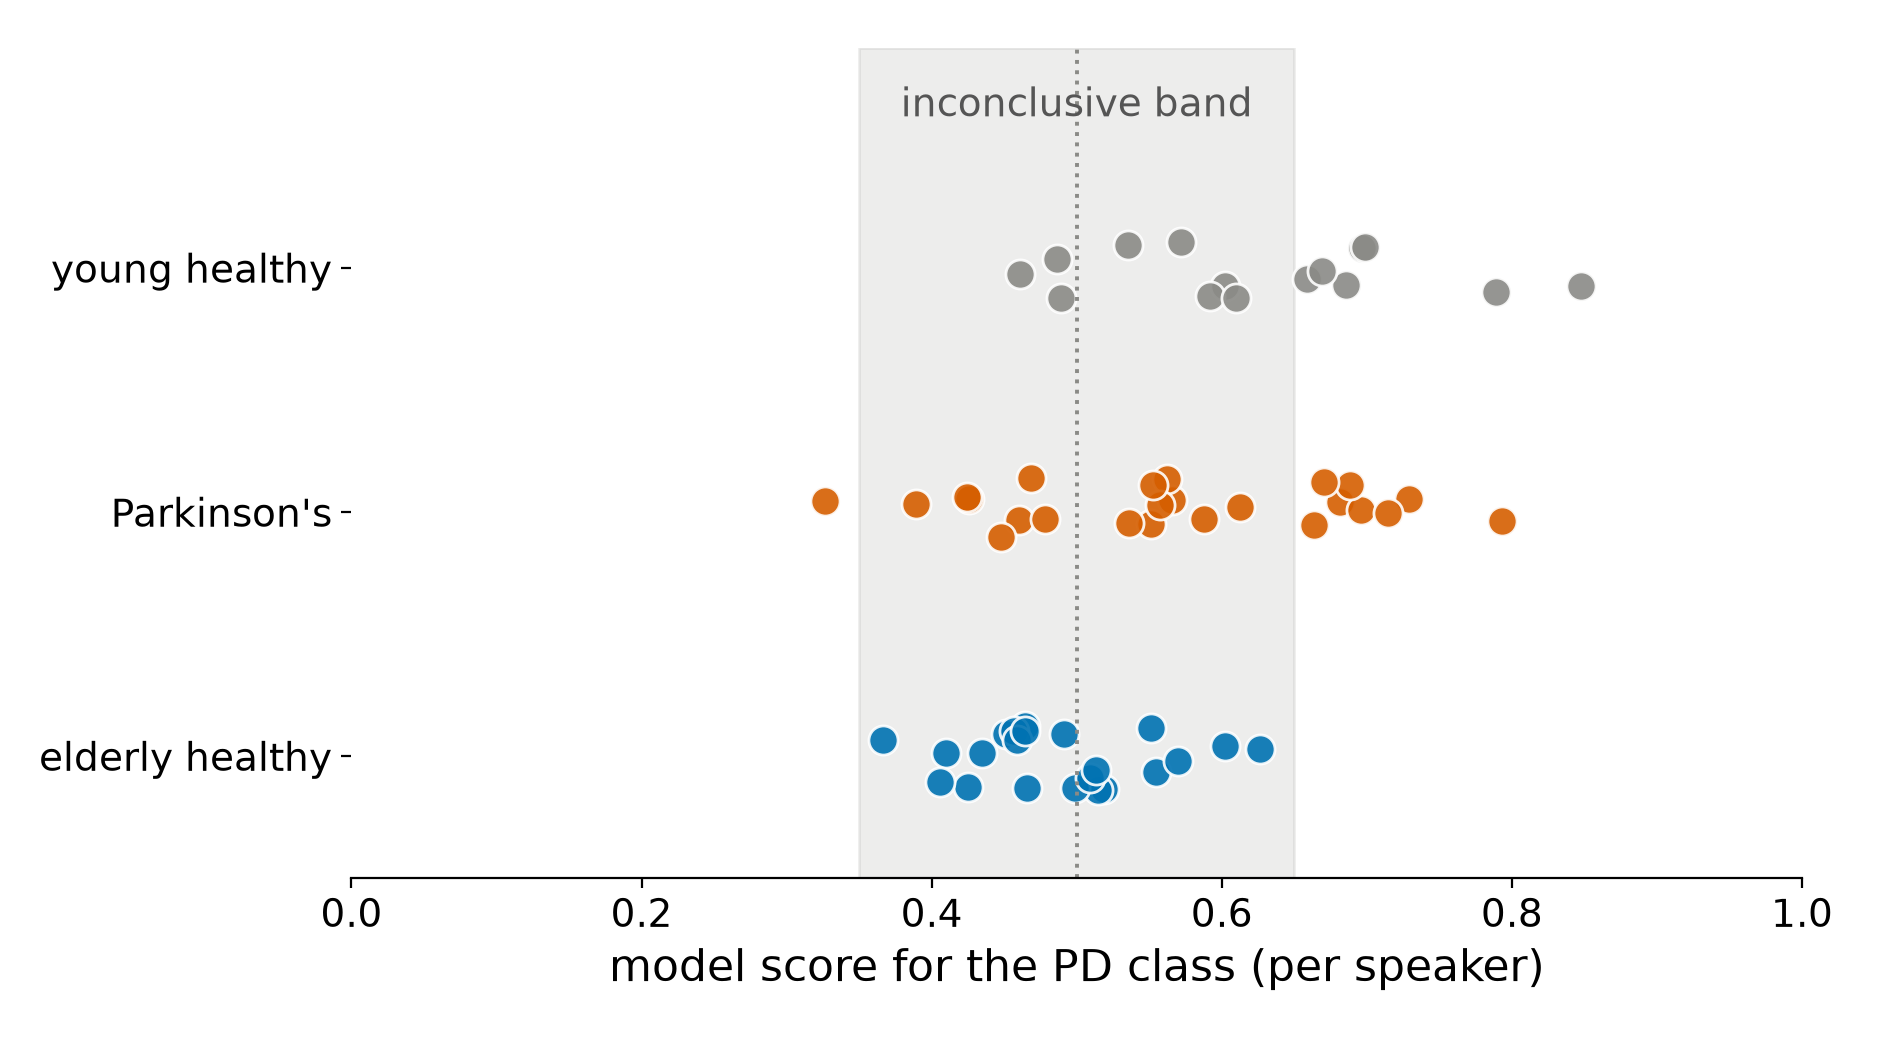
\includegraphics[width=\textwidth]{figs/external_slide.png}
\end{columns}
\end{frame}

% ===== 14 — ACT 5 =====================================================
\begin{frame}{A system that refuses to guess}
\begin{columns}[c]
\column{0.40\textwidth}\centering
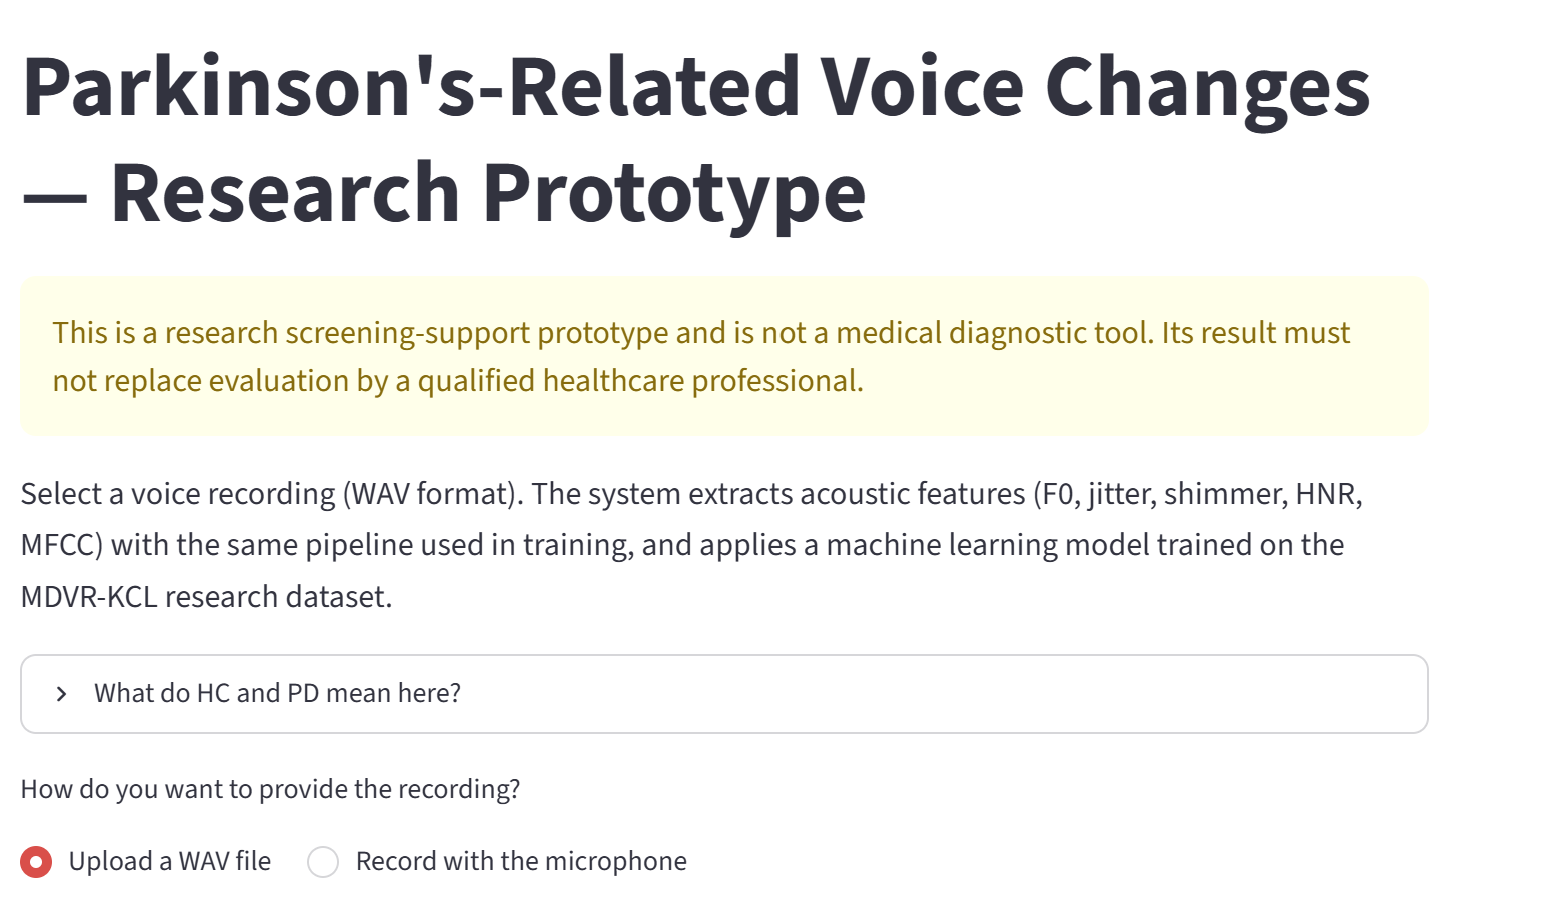
\includegraphics[width=0.92\linewidth]{../figures/app_interface.png}\\[2mm]
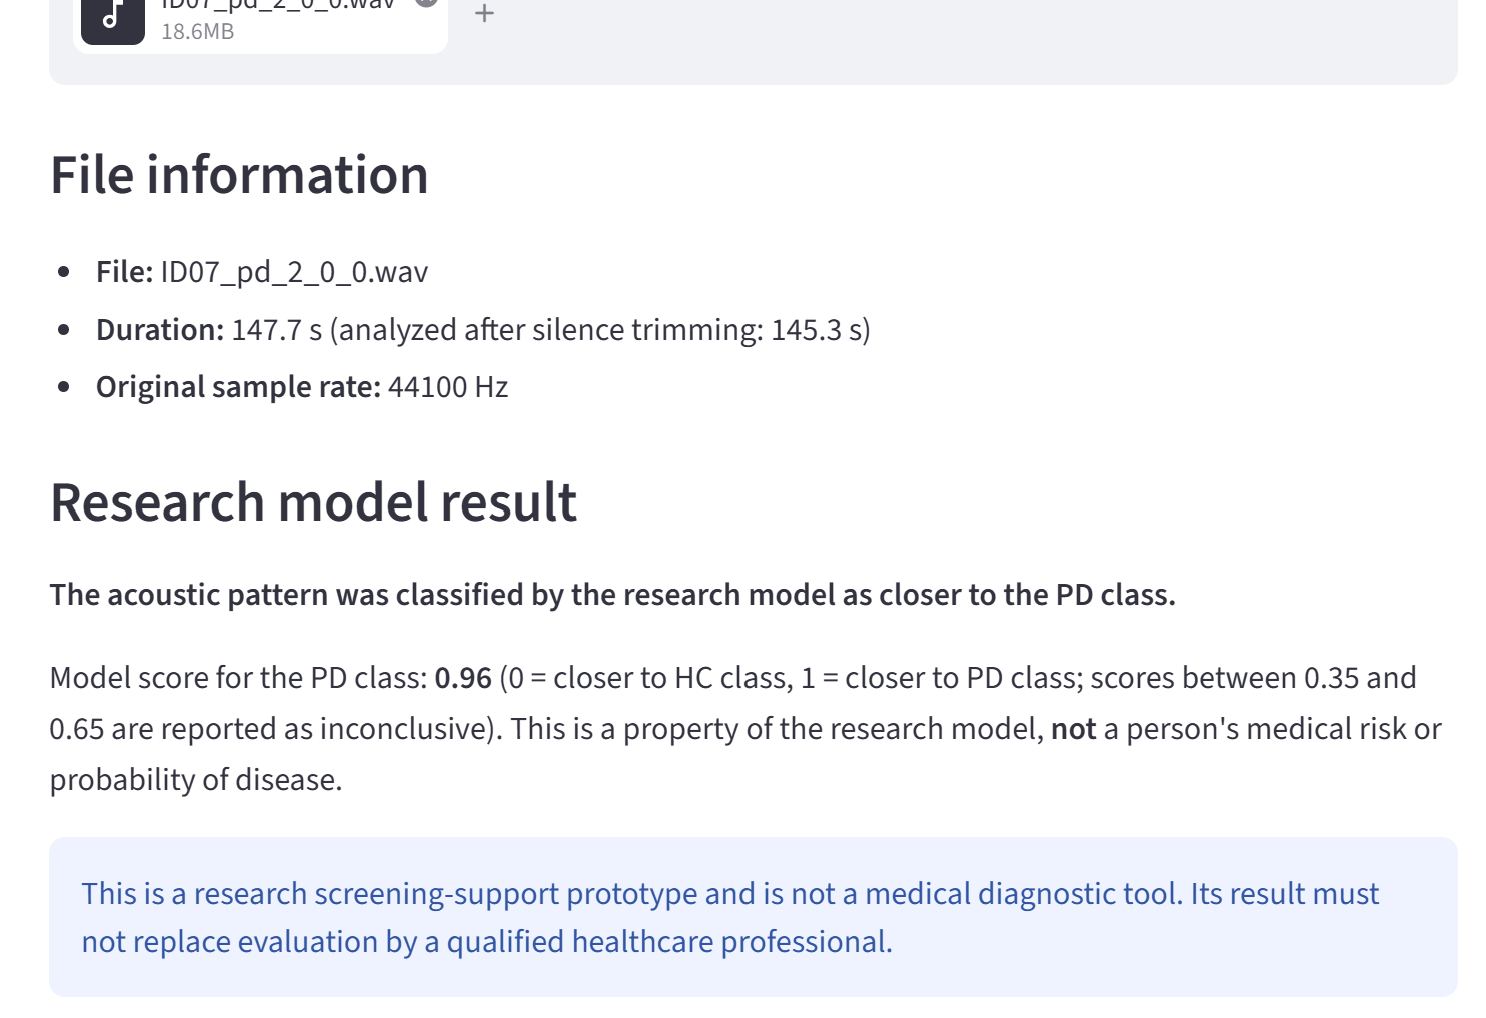
\includegraphics[width=0.92\linewidth]{../figures/app_result.png}
\column{0.56\textwidth}
\begin{itemize}
  \item scores 0.35--0.65 $\Rightarrow$ ``inconclusive''
  \item \textcolor{honest}{100\% of elderly healthy Italian speakers}
        landed there
  \item declining to answer is a feature
\end{itemize}
\end{columns}
\end{frame}

% ===== DEMO MARKER (optional) =========================================
\begin{frame}{\textcolor{soft}{Optional: live demonstration}}
\vspace{4mm}
\begin{itemize}
  \item safest demo: a corpus recording, command line
  \item analysis takes about one minute
  \item fallback: the screenshots on the previous slide carry the same
        content
\end{itemize}
\vspace{4mm}
\centering{\small\textcolor{soft}{skip this slide if time is short}}
\end{frame}

% ===== 15 =============================================================
\begin{frame}{What this is --- and is not}
\vspace{1mm}
\begin{itemize}
  \item not a diagnostic tool; many conditions change a voice
  \item 37 subjects, one language, one device
\end{itemize}
\vspace{5mm}
\bigclaim{Validation design moves the number\\more than model
engineering does.}
\vspace{2mm}
\centering An honest \textcolor{honest}{\textbf{0.822}} is worth more
than an inflated one.
\end{frame}

% ===== END MARKER =====================================================
\begin{frame}[c]{}
\bigclaim{Thank you}
\vspace{4mm}
\centering Questions welcome.
\end{frame}

% ===== BACKUP SLIDES (Q&A only) =======================================
\appendix

\begin{frame}{Backup: why 82\% and not 95\%?}
\begin{itemize}
  \item published 95\%+ figures usually split recordings or windows,
        not people
  \item our own pipeline: 0.909 leaky vs 0.775 honest --- same model
  \item 0.822 is measured on people the model never heard
\end{itemize}
\end{frame}

\begin{frame}{Backup: why not deep learning?}
\begin{itemize}
  \item 37 subjects is far below what deep networks need
  \item examiners can ask this model \emph{which} measurements it used
  \item our small neural network collapsed in the confounder test
        (0.671 $\to$ 0.526)
\end{itemize}
\end{frame}

\begin{frame}{Backup: why balanced accuracy?}
\begin{itemize}
  \item classes are imbalanced: 42 HC vs 31 PD recordings
  \item ``always healthy'': 0.575 accuracy, zero patients found
  \item balanced accuracy gives that model 0.500 --- exposed
\end{itemize}
\end{frame}

\begin{frame}{Backup: why reject the 0.840 ensemble?}
\begin{itemize}
  \item adoption margin $+0.02$ was fixed before any experiment
  \item it won by 0.018; seed-to-seed noise is about $\pm$0.03
  \item picking the most complex of tied variants fits the validation,
        not the problem
\end{itemize}
\end{frame}

\begin{frame}{Backup: can it diagnose Parkinson's?}
\begin{itemize}
  \item no --- and it is not designed to
  \item colds, ageing, smoking, fatigue also change the voice
  \item it reports similarity to dataset groups; clinical evaluation
        stays with clinicians
\end{itemize}
\end{frame}

\begin{frame}{Backup: is 37 subjects too few?}
\begin{itemize}
  \item yes --- it is the dominant limitation, stated openly
  \item mitigated: grouped validation, 3 seeds, spread reported
        ($\pm$0.032)
  \item plus an external test on 61 further speakers
\end{itemize}
\end{frame}

\begin{frame}{Backup: is it detecting male vs female voices?}
\begin{itemize}
  \item absolute pitch encodes speaker sex --- so we removed those four
        features
  \item selected model held: 0.768 $\to$ 0.780
  \item the MLP collapsed (0.671 $\to$ 0.526) and was excluded
\end{itemize}
\end{frame}

\begin{frame}{Backup: hardest technical problem?}
\begin{itemize}
  \item finding confounders that would flatter the results
  \item Italian corpus: every 44.1 kHz file was a patient ---
        bandwidth, not disease
  \item caught at inspection; all audio band-limited to 16 kHz first
\end{itemize}
\end{frame}

\end{document}
